\chapter{Lagrange functions in one dimension}


\section{Introduction}

There are various ways to derive what will be referred to as
Lagrange basis functions (LBFs) or Lagrange functions (LFs) below.
In some references, they are also referred to as discrete variable
representation (DVR) basis functions, especially in papers by Tuckerman's
research group [references needed].

In summary, this is the parameters that are needed to specify a specific
LBFs:
\begin{itemize}

\item For periodic and cluster/box LBFs we need to specify:
\begin{itemize}
\item number of basis functions $N$
\item two end points $a$ and $b$
\end{itemize}

\item For sinc LBFs, we need to specify:
\begin{itemize}
\item number of basis functions $N$
\item grid spacing $h$
\end{itemize}

\end{itemize}


\section{Implementation}

Currently, there is only special module to handle global variables related
to 1D LFs. However, there is a special module to handle 3D LFs, namely
the module \texttt{m\_LF3d} defined in file \texttt{m\_LF3d.f90}.
The relevant global variables for our current discussion are the following.
\begin{fortrancode}
INTEGER :: LF3d_NN(3)
REAL(8) :: LF3d_LL(3)
REAL(8) :: LF3d_AA(3), LF3d_BB(3)
REAL(8) :: LF3d_hh(3)
\end{fortrancode}
Note that, these arrays are of size 3, for each $x$, $y$, and $z$ component.
We will restrict ourself to 1D, and will take only the first element, i.e. the
$x$ direction.
The grid points are stored in array:
\begin{fortrancode}
REAL(8), ALLOCATABLE :: LF3d_grid_x(:)
\end{fortrancode}

In the actual code, if there is no name-clash (i.e. no two or more variables with the
same name), we usually use the aliases for these global variables, e.g.:
\begin{fortrancode}
USE m_LF3d, ONLY : NN => LF3d_NN, hh => LF3d_hh
\end{fortrancode}

The relevant subroutines to initialize the grid points for each LFs:
\begin{itemize}
\item \texttt{init\_grid\_1d\_p()}
\item \texttt{init\_grid\_1d\_c()}
\item \texttt{init\_grid\_1d\_sinc()}
\end{itemize}



\section{Initializing grid points for LFs}

The following code fragments initializes 1D periodic LFs:
\begin{fortrancode}
USE m_LF3d, ONLY : grid_x => LF3d_grid_x
IMPLICIT NONE
INTEGER :: N, i
REAL(8) :: L
! Initialize the basis functions
ALLOCATE( grid_x(N) )
CALL init_grid_1d_p( N, -0.5d0*L, 0.5d0*L, grid_x )
WRITE(*,'(1x,A,I5)') 'N = ', N
WRITE(*,'(1x,A,F18.10)') 'L = ', L
WRITE(*,'(1x,A,F18.10)') 'Grid spacing = ', grid_x(2) - grid_x(1)
WRITE(*,*) 'Grid points for periodic LF'
DO i = 1,N
  WRITE(*,'(1x,I5,F18.10)') i, grid_x(i)
ENDDO
DEALLOCATE( grid_x )
\end{fortrancode}

A complete example code can be found in file \texttt{tests/init/ex\_init\_1d.f90}.


\section{Plotting the basis functions}

The relevant subroutines used for this purpose are as follows.
\begin{itemize}
\item \texttt{eval\_LF1d\_p()}
\item \texttt{eval\_LF1d\_c()}
\item \texttt{eval\_LF1d\_sinc()}
\end{itemize}

Plots of periodic, cluster/box, and sinc LFs are
shown in Figure \ref{fig:LF1d_p_5}, \ref{fig:LF1d_c_5}, and
\ref{fig:LF1d_sinc_5} respectively.

\begin{figure}[h]
{\centering
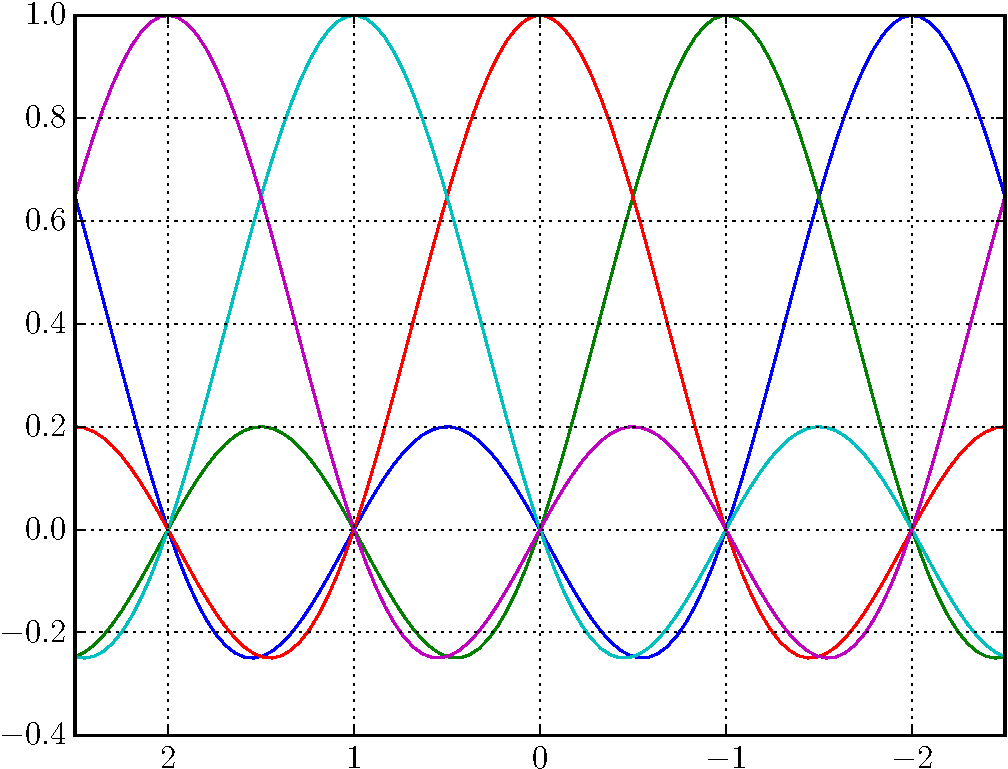
\includegraphics[width=0.5\textwidth]{../../tests/plot_1d/LF1d_p.pdf}
\par}
\caption{Periodic LF}\label{fig:LF1d_p_5}
\end{figure}

An example program which can produce plot data for these figures can be
found in \texttt{../../tests/plot\_1d/ex\_plot\_1d.f90}.

\begin{figure}[h]
{\centering
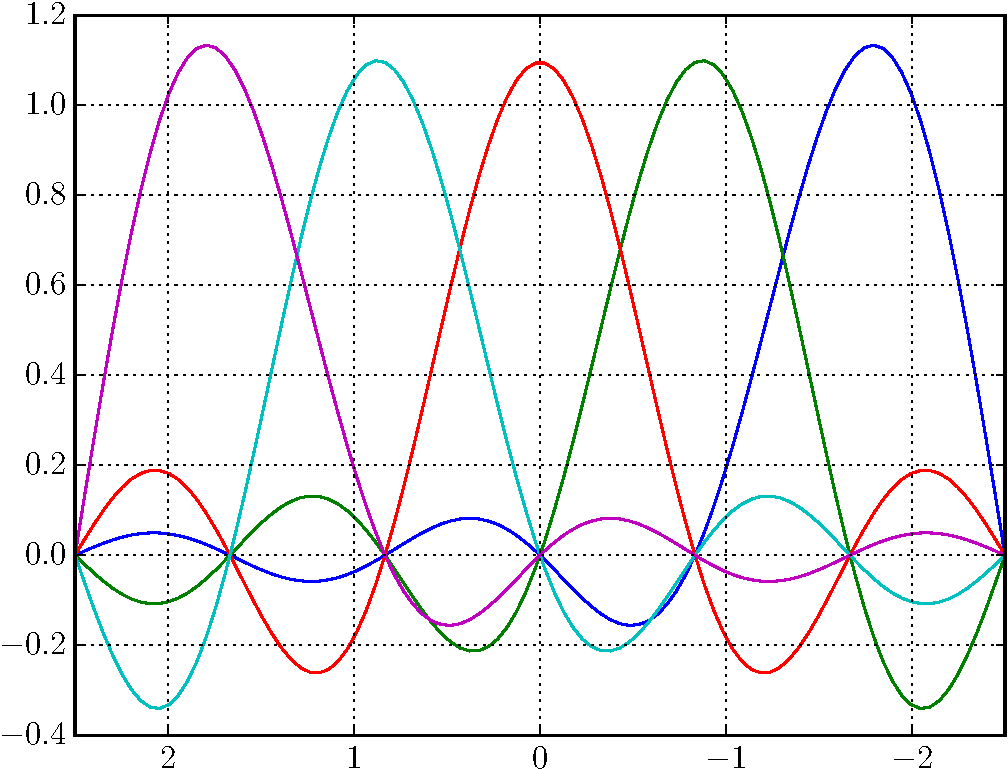
\includegraphics[width=0.5\textwidth]{../../tests/plot_1d/LF1d_c.pdf}
\par}
\caption{Cluster/box LF}\label{fig:LF1d_c_5}
\end{figure}

The following Python script were used to plot the resulting data:
\begin{pythoncode}
import numpy as np
import matplotlib.pyplot as plt
import os
from matplotlib import rc
rc('font',**{'family':'serif', 'size':16})
rc('text', usetex=True)
types = ['sinc', 'c', 'p']
NBASIS = 5
for t in types:
    dat1 = np.loadtxt('LF1d_' + t + '.dat')
    plt.clf()
    for ibf in range(1,NBASIS+1):
        plt.plot( dat1[:,0], dat1[:,ibf] )
    plt.xlim( dat1[-1,0], dat1[0,0] )
    plt.grid()
    FIPLOT = 'LF1d_' + t + '.pdf'
    plt.savefig(FIPLOT)
    os.system('pdfcrop ' + FIPLOT + ' ' + FIPLOT)
\end{pythoncode}

\begin{figure}[h]
{\centering
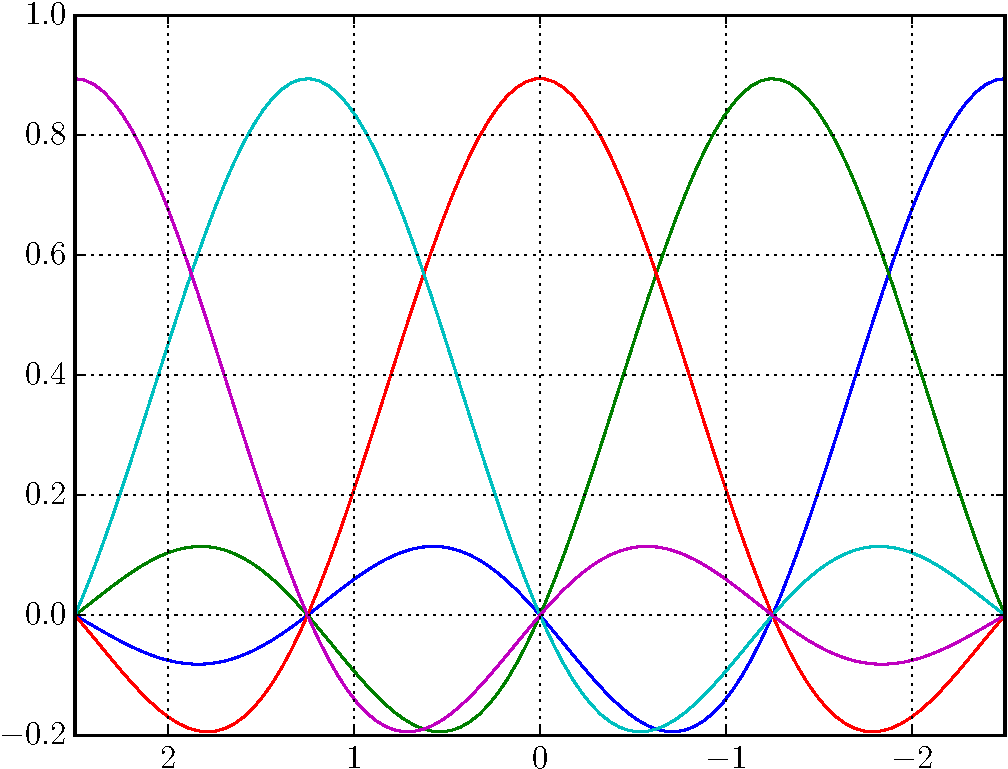
\includegraphics[width=0.5\textwidth]{../../tests/plot_1d/LF1d_sinc.pdf}
\par}
\caption{Sinc LF}\label{fig:LF1d_sinc_5}
\end{figure}


\section{Basis function expansion}

We can expand any "appropriate" function $f(x)$ using LFs:
\begin{equation}
f(x) = \sum_{i}^{N} c_{i} \varphi_{i}(x)
\end{equation}
with $c_{i} = f(x_{i}) \sqrt{\Delta}$

also can use notation $h = \Delta = L/N$

Directory: \texttt{expand_1d_p}





\section{Approximating integrals}

Integral can be approximated as
\begin{equation}
\int f(x)\,\mathrm{d}x \approx \Delta x \sum_{i} f(x_{i})
\end{equation}

Directory: \texttt{integ_1d}
